\documentclass[10pt,a4paper,twocolumn,twoside]{article}
\usepackage[utf8]{inputenc}
\usepackage[provide=*]{babel}
\usepackage{graphicx}
\usepackage{fancyhdr}
\usepackage{times}
\usepackage{titlesec}
\usepackage{multirow}
\usepackage{lettrine}
\usepackage{microtype}
\usepackage{amsmath}
\usepackage{hyperref}
\urlstyle{same}
\usepackage[top=2cm, bottom=1.5cm, left=2cm, right=2cm]{geometry}
\usepackage[figurename=Fig.,tablename=TAULA]{caption}
%\captionsetup[table]{textfont=sc}
\sloppy
\hbadness=10000

\author{\LARGE\sffamily Biel Alavedra Busquet}
\title{\Huge{\sffamily Engraginy: Simulació de Sistemes de Transmissió Mecànica}}

\newcommand\blfootnote[1]{%
  \begingroup
  \renewcommand\thefootnote{}\footnote{#1}%
  \addtocounter{footnote}{-1}%
  \endgroup
}

\titleformat{\section}
{\large\sffamily\scshape\bfseries}
{\textbf{\thesection}}{1em}{}

\begin{document}

\fancyhead[LO]{\scriptsize BIEL ALAVEDRA BUSQUET: ENGRAGINY}
\fancyhead[RO]{\thepage}
\fancyhead[LE]{\thepage}
\fancyhead[RE]{\scriptsize EE/UAB TFG INFORMÀTICA: ENGRAGINY (MECÀNICA I LOGÍSTICA)}

\fancyfoot[CO,CE]{}

\fancypagestyle{primerapagina}
{
   \fancyhf{}
   \fancyhead[L]{\scriptsize TFG EN ENGINYERIA INFORMÀTICA, ESCOLA D'ENGINYERIA (EE), UNIVERSITAT AUTÒNOMA DE BARCELONA (UAB)}
   \fancyfoot[C]{\scriptsize Gener de 2026, Escola d'Enginyeria (UAB)}
}

\renewcommand{\headrulewidth}{0pt}
\renewcommand{\footrulewidth}{0pt}
\pagestyle{fancy}

\twocolumn[\begin{@twocolumnfalse}

\maketitle

\thispagestyle{primerapagina}

\begin{center}
\parbox{0.915\textwidth}
{\sffamily
\textbf{Resum--}
Engraginy és un videojoc 3D que busca simular sistemes de transmissió mecànica, fent ús d'engranatges, eixos i altres mecanismes amb l'objectiu de construir cadenes de producció i fàbriques. El nucli del projecte és el sistema de potència i transmissió mecànica, basat en grafs que fa ús de càlcul vectorial i senyals per actualitzar el sistema quan es requereix. A més d'un sistema de transport de materials basat en simulacions físiques. Tots aquests sistemes han estat dissenyats i pensats per oferir una experiència totalment reactiva.

\textbf{Paraules clau-- } Godot, Videojoc, Grafs, GDScript, Logística, Simulació 3D.

\bigskip

\textbf{Abstract--}
Engraginy is a 3D video game that seeks to simulate mechanical transmission systems, utilizing gears, shafts, and other mechanisms with the goal of building production chains and factories. The core of the project is the power and mechanical transmission system, based on graphs that use vector calculation and signals to update the system as required. Additionally, it features a material transport system based on physical simulations. All these systems have been designed to offer a fully reactive experience.

\textbf{Keywords-- } Godot, Videogame , Graphs, GDScript, Logistics, 3D Simulation.
}

\bigskip

{\vrule depth 0pt height 0.5pt width 4cm\hspace{7.5pt}%
\raisebox{-3.5pt}{\fontfamily{pzd}\fontencoding{U}\fontseries{m}\fontshape{n}\fontsize{11}{12}\selectfont\char70}%
\hspace{7.5pt}\vrule depth 0pt height 0.5pt width 4cm\relax}

\end{center}

%\bigskip
\end{@twocolumnfalse}]

\blfootnote{$\bullet$ E-mail de contacte: biel.alavedra@gmail.com}
\blfootnote{$\bullet$ Menció: Computació}
\blfootnote{$\bullet$ Treball tutoritzat per: Enric Marti Godia}
\blfootnote{$\bullet$ Curs 2025/26}

\section{Introducció}

\lettrine[lines=3]{E}{l} projecte Engraginy neix de la voluntat d'explorar mecàniques de joc més físiques dins del gènere de l'automatització. Mentre que títols referents com \textit{Factorio} \cite{factorio} i \textit{Satisfactory} \cite{satisfactory} utilitzen l'electricitat com un recurs binari o simplificat, aquest treball proposa una xarxa de potència mecànica on cada component (engranatges, eixos, cintes) afecta el rendiment de les cadenes de producció segons les lleis de la cinemàtica bàsica.

L'objectiu principal és la creació d'un sistema modular i extensible en el motor \textit{Godot} \cite{godot} que permeti al jugador construir xarxes de potència complexes. Per aconseguir aquest objectiu es dissenya, implementa i testeja un videojoc del gènere d'automatització, que compleixi amb els següents requisits:
\begin{itemize}
\item Joc en primera persona
\item Menú de construcció que mostri tots els elements que es poden construir: engranatges, eixos, generadors, etc.
\item Sistema de càrrega i guardat de partida
\item Sistema de construcció basat en graella
\item Sistema de simulació de transmissió mecànica
\item Sistema de transport d'objectes
\end{itemize}

El repte tecnològic a afrontar resideix en la propagació dinàmica de la rotació en un entorn 3D, requerint l'ús de càlculs vectorials per determinar la viabilitat de les connexions, i les direccions de transmissió.

La motivació principal per al desenvolupament d'aquest projecte és aprendre com funciona el desenvolupament d’un videojoc. Estudiar el cicle de vida i les diferents fases necessàries per a crear un videojoc. Els referents estudiats a l’hora de desenvolupar el projecte són videojocs com \textit{Factorio}, \textit{Satisfactory}, \textit{Dyson sphere program} (DSP) \cite{dsp}, \textit{Shapez} \cite{shapez}, i \textit{Minecraft: Create Mod} \cite{create} (una modificació del joc no oficial).

D'entre els referents analitzats, cal destacar \textit{DSP} i \textit{Satisfactory}, dos videojocs que sobresurten per la seva capacitat d'immersió i estimulació  lògica. Aquests títols exemplifiquen com d'entretingut i mentalment activador pot ser el gènere. El \textit{DSP} és un joc molt més ambiciós, s'inicia en un petit  satèl·lit dins d’un cúmul d’estrelles generat aleatòriament, i acaba quan el jugador és capaç de navegar entre sistemes solars i construeix una esfera de Dyson \cite{dyson}. Tot això amb una perspectiva isomètrica que facilita la supervisió i atorga un gran control de tot allò que es construeix. En la fig. \ref{fig:dsp} es mostra un exemple de com es veu i es construeix en el joc.

\begin{figure}[!ht]
\centering
    \includegraphics[width=0.5\textwidth]{img/dsp.png}
    \caption{Exemple de com el jugador veu el joc (vista isomètrica)}
    \label{fig:dsp}
\end{figure}

En el \textit{Satisfactory} l’objectiu és completar un ascensor espacial. Es comença en un planeta (el qual sempre és el mateix, el mapa és prefixat). Aquest joc és en primera persona, i totes les màquines que es construeixen són gegantines. Això impedeix una visió completa d’allò que es construeix. En quantitat de màquines les construccions són sempre més petites i molt més lentes de construir. S'observa en la fig. \ref{fig:satisfactory} la gran diferència entre les dues captures, mentre en una es presenta una vista sencera del procés, en la segona hi ha una visió més limitada, però molt més immersiva.

\begin{figure}[!ht]
\centering
    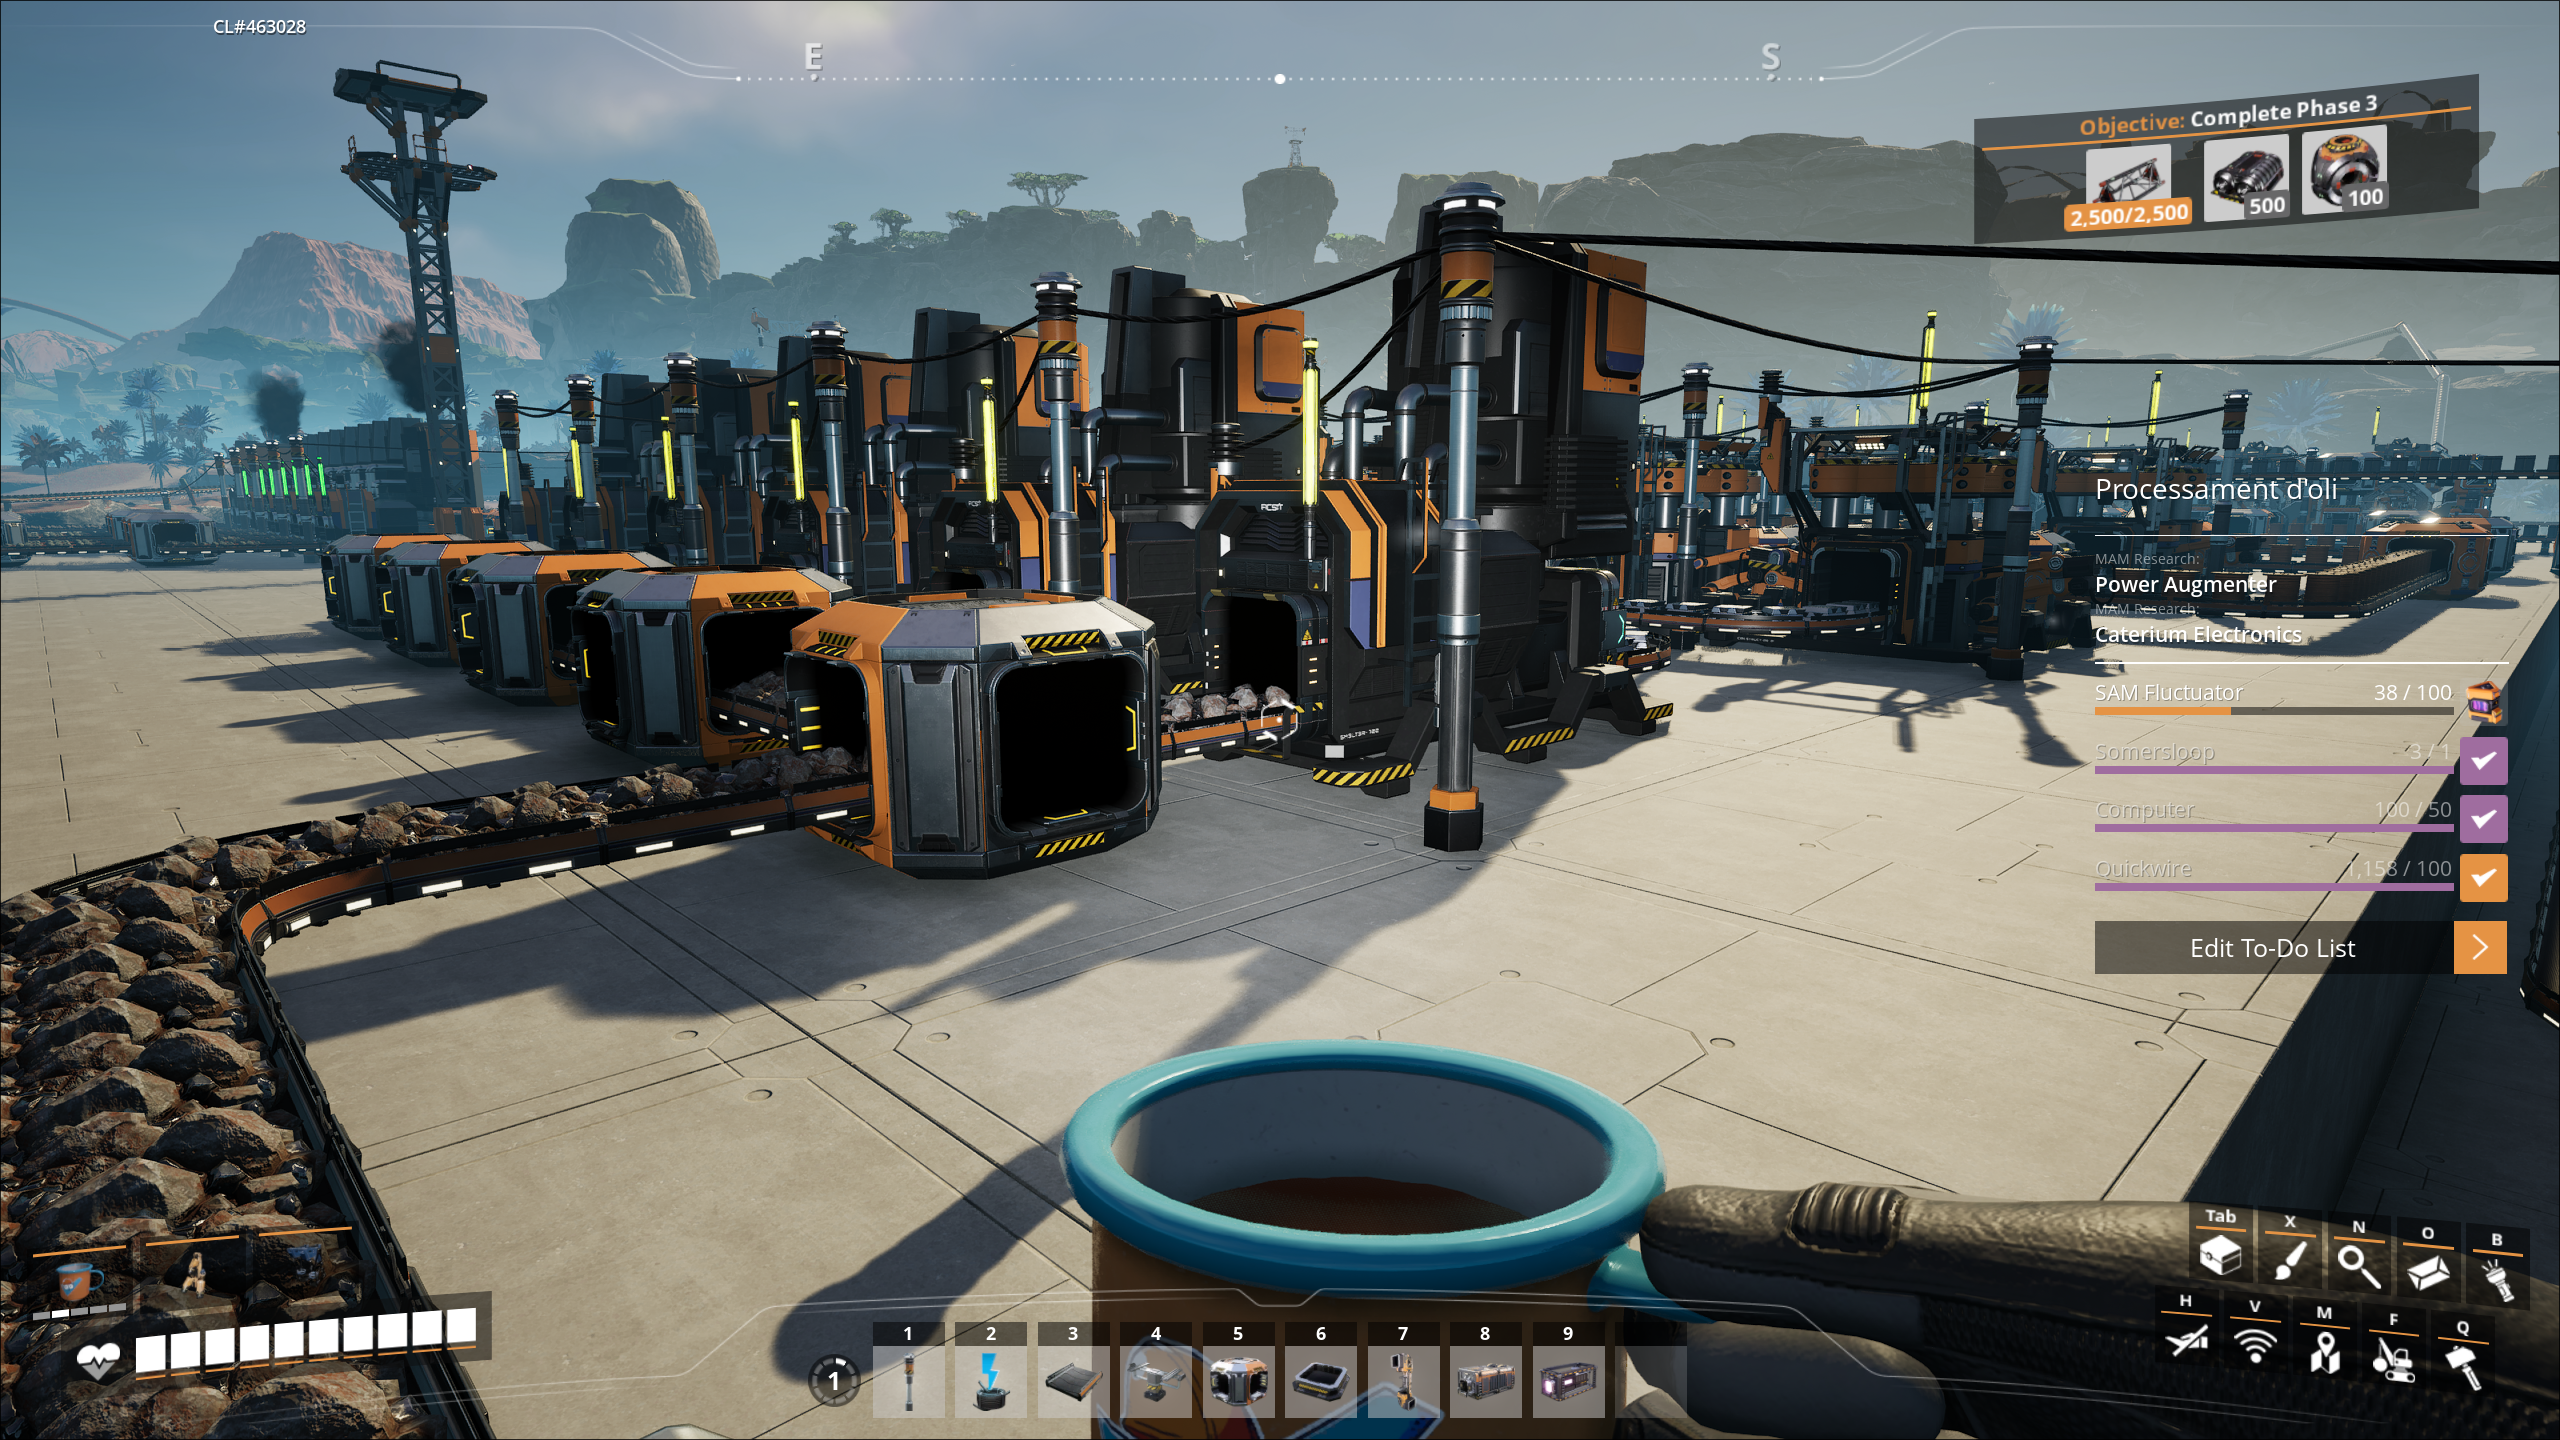
\includegraphics[width=0.5\textwidth]{img/satisfactory.png}
    \caption{Exemple de com el jugador veu el joc (primera persona)}
    \label{fig:satisfactory}
\end{figure}

L'objectiu és desenvolupar un sistema amb mecàniques més similars a \textit{Satisfactory}, ja que aquesta visió en primera persona dona un control més granular de les construccions a petit nivell, i encaixa molt millor amb les mecàniques a incorporar de \textit{Minecraft: Create mod}. En la majoria dels jocs de l’estil una part molt important és la generació d’energia. És molt ineficient fer fàbriques més grans si no es tenen els recursos per mantenir-les. Tant \textit{DSP}, \textit{Factorio} i \textit{Satisfactory} utilitzen energia elèctrica, sigui solar, eòlica, carbó o nuclear. Tots aquests generadors s’acaben connectant a la xarxa elèctrica per donar energia a totes les màquines. En canvi, el \textit{Minecraft: Create mod} requereix que tot sigui alimentat per energia cinètica, fent ús d’eixos, engranatges grans i petits, cadenes, corretges de transmissió, etc. Com l'objectiu és fer un joc amb una ambientació prerevolució industrial, i no del tipus fantàstic, aquesta sembla ser la millor opció per aconseguir-ho. També això afegeix totes les mecàniques d’haver de connectar les màquines, no només a una velocitat concreta, ja que algunes seran direccionals, com les cintes per transportar material.

D’entre tots els gèneres de videojocs perquè s'ha escollit l'automatització? Aquest és un gènere que segueix molt la filosofia d'un programador, o en general la de tots els enginyers: dividir i vèncer. L’inici d’aquests jocs és senzill, amb unes poques màquines cal fer processos simples. Per exemple, amb un extractor de recursos automàtic i cal processar els recursos en brut per tal d’obtenir el recurs processat (de mena de ferro a lingots de ferro). Però això ràpidament canvia, agafant d’exemple el joc \textit{DSP}. Si es vol fer una placa de circuits es necessita un forn de fosa que converteixi el mena de ferro a plaques de ferro, un altre forn de fosa que converteixi coure en brut a plaques de coure i un assemblador que agafi aquests dos materials i els converteixi en la placa de circuits. Això és només un dels primers passos, on cada vegada es disposa de més i més materials diferents, processos diferents i els objectes requerits són cada vegada més complexes. Per força no es poden afrontar tots aquests problemes simultàniament, cal dividir els problemes en mòduls que es puguin replicar cada vegada que calgui per a resoldre aquell problema.

Dins de la comunitat de fans d’aquest gènere de videojoc hi ha molts enginyers i gent a què agrada molt optimitzar processos i fer construccions el màxim d’eficients possibles. Per tot això el gènere no és només entretingut, sinó que també en certa manera és educatiu, doncs força al jugador a organitzar-se, pensar formes eficients de construir coses, com connectar les entrades i sortides de totes les fàbriques, calcular que tanta entrada es necessita per la sortida objectiva i construir d’acord amb això. Per completar el joc cal ser organitzat, metòdic i pensar en solucions segons el problema que es tingui.

\section{Conceptes bàsics de Godot}

Prèviament a la descripció tècnica del projecte és necessari explicar el funcionament de tres conceptes clau: Nodes, Escenes i Senyals. Aquests termes apareixeran recurrentment al llarg de l'article.
Pel fet d'utilitzar Godot l'estructura interna del projecte ha de seguir els requisits del motor. Això implica fer ús del sistema de nodes i escenes per crear tots els objectes, i aprofitar els senyals per simplificar connexions entre objectes.

\subsection{Nodes}
Cada element del joc és un node amb unes propietats i funcions diferents. Hi ha tres famílies principals: nodes 3D, nodes 2D i nodes de "GUI" (Interfície d'Usuari).

Dins de la família de nodes 3D, que són els més rellevants per la simulació, hi ha exemples com:
\begin{itemize}
\item Camera3D
\item StaticBody3D
\item MeshInstance3D (per als models visuals)
\item CollisionShape3D (per a les físiques)
\item RayCast3D (per a detectar objectes)
\end{itemize}
Tots aquests nodes hereten de la classe base \texttt{Node3D}. D'aquesta classe obtenen les propietats essencials de qualsevol objecte a l'espai: la posició, la rotació i l'escala.

Els nodes de "GUI" (\texttt{Control}) permeten la creació d'interfícies d’usuari on s'utilitza l’estructura jeràrquica per encapsular cada element d'interfície com ara:
\begin{itemize}
\item Container
\item Label
\item TextureRect
\item Button
\item Panel
\item ItemList
\item etc.
\end{itemize}
Els nodes 2D no són rellevants per al projecte, però molts d'ells tenen equivalents en els nodes 3D.

\subsection{Escenes}
Les escenes seran definides per l’usuari i són una col·lecció de nodes de qualsevol classe. Una escena pot ser el jugador, la interfície d’usuari o un nivell sencer d’un joc. L'organització i contingut d'aquestes escenes respon a les decisions de disseny i arquitectura del programari. Aquestes escenes es poden instanciar dins d'altres escenes, la qual cosa permet dividir problemes grans en mòduls més petits i manejables.

\begin{figure}[!ht]
\centering
    \includegraphics[width=0.5\textwidth]{img/PlayerScene.png}
    \caption{Escena del jugador amb la jerarquia de nodes}
    \label{fig:player-scene}
\end{figure}

En l'escena que conté el jugador, fig. \ref{fig:player-scene}, hi ha com a node pare un \texttt{PlayerCharacter} (node propi, hereta de la classe base \texttt{CharacterBody3D}), amb 5 fills, el punt d'ancoratge de la càmera (\texttt{CameraHolder}), la caixa de col·lisions del personatge (\texttt{Hitbox}), els \texttt{RayCast3D} (\texttt{Raycasts}), el \texttt{Model} i la màquina d’estats encarregada del control del personatge. Aquesta màquina d’estats està iniciada amb nodes buits, que són la classe base per a tots els objectes de Godot, i no tenen propietats especials. Al lateral s'observa una icona amb un pergamí, que indica que hi ha un script vinculat al node. Si està en gris vol dir que aquest script és heretat, compartit amb altres nodes de la mateixa classe. Si és blanc indica que el node té un script únic.

\subsection{Senyals}

Els senyals permeten connectar diferents nodes i escenes sense necessitat de conèixer exactament l’estructura de l'escena ni haver de fer referència al node directament. Aquests senyals són missatges que els nodes poden emetre; els altres nodes es poden connectar a aquest senyal i executar una funció quan reben el missatge. Aquests missatges es poden emetre directament per codi, poden respondre a accions del jugador o a canvis en l'estructura de l'escena. Aquest sistema redueix molt les dependències i fa el codi més modular, ja que s'eviten referències directes entre escenes. Per explicar com s'utilitza aquest sistema es pren com a exemple el mecanisme que s'ha desenvolupat per interactuar amb objectes.

\begin{figure*}[!ht]
\centering
    \includegraphics[width=0.9\textwidth]{img/InteractCastCode.png}
    \caption{Fragment de codi de l’objecte PlayerCharacter que conté les funcions per emetre senyals}
    \label{fig:interact-cast-code}
\end{figure*}

En aquest fragment de codi, fig. \ref{fig:interact-cast-code}, es defineixen les funcions utilitzades per emetre els tres senyals d'interacció amb l’entorn: \texttt{unfocused}, \texttt{focused} i \texttt{interacted}. La funció \texttt{interact\_cast()} s'executa en cada fotograma del joc per comprovar si s'està interactuant amb algun objecte.
El primer pas és obtenir l'objecte que el jugador està mirant directament. Per fer-ho, s'emet un \texttt{RayCast3D} des de l’origen de la càmera fins a una certa distància i es retorna el primer objecte amb el qual col·lideix mitjançant la funció \texttt{make\_cast\_query()}.

Si l'objecte retornat és el mateix que en el fotograma anterior, no es fa res. En cas contrari, es verifica si l’objecte anterior tenia definit el senyal \texttt{unfocused}. Si no estigués definit, vol dir que amb aquell objecte no es podia interactuar; si hi és, s'emet el senyal. Tot seguit, si el nou objecte que el jugador està mirant té el senyal \texttt{focused}, s'emet per indicar que ha rebut el focus.

D'altra banda, la funció \texttt{interact()} només s’executa quan el jugador prem el botó d’interactuar. El procediment és similar: es comprova que l’objecte tingui el senyal \texttt{interacted} i, en cas afirmatiu, s'emet.

Per gestionar la resposta a aquests senyals, els objectes interactius disposen d'un node fill anomenat \texttt{InteractionComponent}. Aquest conté l'script encarregat de processar els senyals i cridar les funcions adients de l’objecte pare. Aquest component ha de ser fill d’un node \texttt{StaticBody3D}, ja que la funció \texttt{make\_cast\_query()} requereix cossos físics per detectar la interacció.
Finalment, en l’objecte \texttt{InteractionComponent} es busca el node pare i es connecten aquests senyals amb les funcions \texttt{in\_range}, \texttt{not\_in\_range} i \texttt{on\_interact} definides en la lògica de l'objecte.

\section{Desenvolupament}

\begin{figure*}[!ht]
\centering
    \includegraphics[width=0.9\textwidth]{img/DiagramaModuls.png}
    \caption{Diagrama de mòduls}
    \label{fig:module-diagram}
\end{figure*}

El programari s'ha estructurat seguint els principis de la programació orientada a objectes (POO) mitjançant el sistema de nodes de Godot. En el diagrama de mòduls de la fig. \ref{fig:module-diagram} es poden veure les classes més importants del projecte. Aquest diagrama no és una versió completa, però conté els components i classes més importants del projecte.

A la dreta s'observa l'oval que representa al jugador, això no és una classe, però indica allò que el jugador controlarà directament.

El jugador controla directament tres components: el \texttt{PlayerCharacter} és l'avatar del jugador, controla el moviment i les col·lisions, el \texttt{CameraObject} s'encarrega del control de càmera i de com el jugador veu el món, i finalment totes les GUI. Depenent del context i amb diferents entrades el jugador podrà controlar aquesta part, per exemple, amb la tecla "TAB" i podrà obrir i tancar el \texttt{BuildingMenu}.

Aquest \texttt{BuildingMenu} conté un llistat amb tots els possibles objectes que es poden construir, separats en quatre pestanyes (Producció, energia, fonaments i decoració), per a una millor organització. Des d'aquest menú el jugador pot fer servir el ratolí per arrossegar objectes a la \texttt{HotBar}. Aquesta barra d'accés directe conté la lògica per a la construcció d'objectes. Prement una de les tecles 1-9 es selecciona una de les seves caselles i si aquesta conté un objecte el joc mostra una previsualització de \texttt{Building}. Aquesta serà verda si l'objecte està en una posició vàlida i vermella si està col·lidint amb un altre objecte i no pot ser col·locada.

La classe \texttt{Building} és la classe base de qualsevol objecte que el jugador podrà col·locar. Conté tota la lògica per gestionar les col·lisions, l'entrada amb l'escena, la inicialització de variables necessàries i els mètodes necessaris per interactuar i permetre al jugador eliminar l'objecte.

Per gestionar aquesta última part s'utilitza la classe \texttt{InteractionComponent}. Aquest és un node que s'afegeix a l'escena de tot \texttt{Building}, que fent ús de senyals informa l'objecte si el jugador l'està mirant (el cursor del centre de la pantalla està just a sobre l'objecte i el jugador no està massa lluny de l'objecte), l'ha deixat de mirar, o el jugador ha executat alguna entrada especifica com pressionar la tecla "R" per eliminar l'objecte.

La classe \texttt{PowerNode} hereta de la classe \texttt{Building}. Aquesta és la classe que gestiona totes les connexions lògiques per a tots els elements del sistema de potència. Aquests nodes formen un graf no dirigit on cada node coneix únicament els seus veïns. La classe \texttt{PowerGridManager} gestiona la resolució de conflictes dins la xarxa, els canvis de velocitat o l'aturada completa d'aquella xarxa si se supera el límit de potència d'aquella xarxa. Tots aquests canvis són executats només quan hi ha un canvi a la xarxa, i només es recalcula aquella xarxa en concret. Així s'evita càrrega computacional innecessària en comprovar canvis on no n'hi ha. Aquests elements de la xarxa són tot un conjunt de classes més petites que hereten de \texttt{PowerNode}, com: \texttt{Shaft}, \texttt{Cog}, \texttt{Machine}, \texttt{Generators}, etc.
Finalment per gestionar totes aquestes connexions entre \texttt{PowerNodes} s'utilitzen els \texttt{PowerNodePort}, que s'encarreguen d'avisar al node quan un altre node ha entrat en el rang de connexió i quan un node marxa d'aquest rang.

A continuació s'expliquen els sistemes més importants del projecte. Cada sistema gestiona una part independent del videojoc i presenten un baix acoblament entre ells.
\begin{itemize}
\item Lògica de transmissió mecànica
\item Lógistica i transport d'ítems
\item Interfícies d'usuari
\item Construcció i interacció amb objectes
\item Guardar i carregar escenaris
\end{itemize}

\subsection{Lògica de Transmissió Mecànica}
El sistema de transmissió mecànica és una adaptació del sistema existent a \textit{Minecraft: Create mod}. A continuació es farà un llistat de les especificacions del sistema, i com es comporta sota cada cas específic.
\begin{itemize}
\label{Objectives-mech-trans}
\item Tota connexió d’un eix ha de mantenir direcció i velocitat.
\item Tota connexió d’un engranatge ha d’invertir la direcció.
\item Connectar un engranatge petit a un gran a través de les dents de l’engranatge ha d'augmentar la velocitat, a l’invers la velocitat es redueix.
\item La xarxa no pot superar el límit d’energia subministrada per tot el conjunt de generadors connectats.
\item En cas de superar el límit tot el sistema s’ha d’aturar a l’instant.
\item En cas de tornar a estar per sota del límit, el sistema ha d’entrar en funcionament a l’instant.
\item En cas que un node tingui incoherències en els seus ports connectats s’ha d’eliminar automàticament.
\end{itemize}
La classe principal d’aquest sistema és \texttt{PowerNode}. D’aquesta classe hereten tots els elements de la xarxa que s'afegiran. Cada \texttt{PowerNode} tindrà mínim un \texttt{PowerNodePort}. Aquests ports són àrees ubicades allà on es vol que el \texttt{PowerNode} tingui un punt de connexió. Perquè es connectin dos \texttt{PowerNode} els dos ports han d'estar en contacte. Aquest port té quatre propietats molt importants: la direcció de gir respecte al node, el modificador de velocitat, el tipus de port que és, i a quins altres ports es pot connectar.

En els següents subapartats s'explica el funcionament principal dels \texttt{PowerNode}:
\begin{itemize}
\item Quines parts formen els \texttt{PowerNode} i com s'implementen.
\item Funcions del gestor central \texttt{PowerGridManager} i com funciona.
\item Com funciona el procés de càlcul de velocitats entre diferents nodes.
\end{itemize}

\subsubsection{Construcció de les escenes pels \texttt{PowerNode}}

\begin{figure}[!ht]
\centering
    \includegraphics[width=0.5\textwidth]{img/PowerNodePort.png}
    \caption{Exemple de port d'un eix}
    \label{fig:shaft_port}
\end{figure}

En la figura \ref{fig:shaft_port}, es presenta com estan configurats els ports d’un eix bàsic. Respectivament apareixen les propietats: modificador de velocitat ("Ratio Multiplier"), direcció de gir ("Direction Flipper"), tipus de port ("Type") i connexions permeses ("Allow Ports"). Els tipus de port implementats són: "SHAFT\_END", "COG\_SMALL", "COG\_BIG" i "BELT". En cas d’implementar un element que permeti invertir gir s'han d'afegir dos ports, un com el de la figura \ref{fig:shaft_port}, i l’altre amb el "Direction Flipper" a -1. Si es volgués  implementar un element que dupliqués la velocitat de gir s'hauria de modificar el "Ratio Multiplier" a 2.

\begin{figure}[!ht]
\centering
    \includegraphics[width=0.5\textwidth]{img/ShaftScene.png}
    \caption{Exemple de l'escena d'un eix}
    \label{fig:shaft_scene}
\end{figure}

En la figura \ref{fig:shaft_scene} es veu l’exemple de l’eix, amb els dos ports col·locats un a cada extrem de l’objecte. Aquests ports són els petits cubs blaus translúcids situats en els extrems.
Aquests ports hereten de la classe base de Godot \texttt{Area3D}. Com aquesta classe base ja té implementats una sèrie de mètodes que permeten la detecció d'altres objectes en entrar o sortir dins la seva àrea, aquests mètodes faciliten cridar altres funcions en el moment que es produeixi un canvi. Així sempre en detectar un traspàs es cridarà la funció "\_on\_area\_entered()" i quan es detecti que un objecte surt es cridarà la funció "\_on\_area\_exited()".

\subsubsection{\texttt{PowerGridManager} gestor central de transmissió i càlcul de potència}

El \texttt{PowerGridManager} entra en funcionament quan es detecta un senyal que informa d'una modificació en la xarxa. Aquests senyals són enviats quan el \texttt{PowerNode} detecta una connexió o desconnexió vàlida en un dels seus \texttt{PowerNodePort}. Aquesta connexió vàlida llança el senyal "network\_changed", el \texttt{PowerGridManager} recull aquest senyal i comença el procés de recàlcul de la xarxa.

Aquest procés de càlcul comença amb un algoritme "Breadth-first search" ("BFS") \cite{bfs}. Es podria utilitzar també un "Depth-first search" ("DFS") \cite{dfs} per tal de trobar tots els nodes connectats. No hi ha diferència entre l'algorisme "BFS" o el "DFS", però més endavant veurem que cal usar forçosament un "BFS", per tant, ja es té la funció implementada. Una vegada s'obtenen tots aquests nodes es comença la cerca per trobar quins són els generadors de la xarxa, i és a partir d’aquests generadors que es comencen a propagar tots els canvis. Per propagar els canvis s'aplica un altre "BFS". En aquest cas ha de ser aquest algoritme, ja que és preferible que els canvis es propaguin nivell a nivell, que es calculin abans els nodes més pròxims per així detectar els possibles conflictes en els extrems. Per cada node es defineix la seva velocitat com la calculada en el moment d’afegir-lo a la llista de "per visitar", i s'itera per les seves connexions per tal de calcular la velocitat que haurien de tenir per no generar conflictes. En cas de no tenir la connexió una velocitat ja assignada se li assigna la calculada. Si ja tenia una velocitat assignada es comprova que aquestes siguin iguals. En cas de conflicte s'elimina la peça i es torna a començar el procés de càlcul de la xarxa. Si no hi ha conflicte s'afegeix la connexió al llistat de "per visitar". Finalment, quan s'ha acabat amb el càlcul de les velocitats es recorre tota la xarxa per comprovar que la potència és suficient per mantenir la xarxa activa. Tots els generadors sumen les seves potències i els altres nodes resten.

\subsubsection{Càlcul de velocitats}

La part més complexa d’aquest procés és el càlcul de velocitats. Els nodes poden estar situats en qualsevol punt del món i en qualsevol direcció. Per exemple un eix sense girar connectat a un de girat 180 graus presenten una aparença idèntica, però si es fa una assignació directa de velocitat, el segon eix girarà en sentit contrari. Per solucionar això es fan una sèrie de càlculs amb els vectors de direcció de cada element per comprovar com s’ha de comportar aquesta connexió. Aquest comportament serà representat per la variable \textit{Alg}, només tindrà dos possibles valors finals, 1 o -1. Per fer aquest càlcul se seguirà una sèrie de passos, que no s'executen sempre tots. Depenent dels resultats d'operacions anteriors poden canviar els passos que s'executen. El funcionament de tot aquest procés es pot seguir visualment en la fig. \ref{fig:flow-diagram}, que és el diagrama de flux del procés de càlcul que a continuació s'explica.

\begin{figure}[!ht]
\centering
    \includegraphics[width=0.5\textwidth]{img/FlowDiagramSpeedCalcs.png}
    \caption{Diagrama de flux}
    \label{fig:flow-diagram}
\end{figure}

\begin{align}
W_{input} &= W_{conn} \times R_{conn} \times D_{conn} \tag{1}\\
Alg &= \operatorname{sgn}(\vec{A} \cdot \vec{B}) \tag{2} \\
Alg &= \operatorname{sgn}(\vec{S}_{dir} \cdot (1, 1, 1)) \tag{3} \\
\vec{V} &= (\vec{P}_{conn} + \vec{C}_{conn}) - (\vec{P}_{local} + \vec{C}_{local}) \tag{4} \\
Alg &= \operatorname{sgn}((\vec{A} \times \vec{V}) \cdot (-\vec{B} \times \vec{V})) \tag{5} \\
W_{res} &= \frac{W_{input} \times D_{local} \times Alg}{R_{local}} \tag{6}
\end{align}

En la fórmula (1) s'aconsegueix la velocitat d’entrada aparent, $W_{input}$, sense tenir en compte l’alineació dels dos nodes. Els paràmetres són els següents: $W_{conn}$ és la velocitat de rotació del node connectat, $R_{conn}$ és el multiplicador de velocitat del port del node connectat i $D_{conn}$ és la direcció del port del node connectat.

En la fórmula (2) es calcula l’alineació de l’eix de rotació propi, $\vec{A}$, i l’eix de rotació del port connectat, $\vec{B}$. L'alineació es calcula utilitzant el producte escalar entre els dos eixos de rotació. A partir d’aquest punt poden passar dues coses: que el valor de la variable $\text{Alg}$ sigui 0 o 1/-1.

En cas que la variable \textit{Alg} sigui 1/-1 significarà que els dos ports són paral·lels. Si els dos ports són del tipus "SHAFT\_END" la velocitat del port serà la $W_{input}$ multiplicada pel signe de la variable \textit{Alg}. En cas que els ports siguin del tipus "COG" la velocitat serà $W_{input}$ multiplicada pel negatiu de signe de la variable \textit{Alg}, per tal d’invertir la direcció de gir (dos engranatges que es toquin sempre giraran en sentits oposats).

En el cas que la variable \textit{Alg} sigui 0 vol dir que els dos ports són perpendiculars, cas que es dona quan es connecten dos engranatges grans en perpendicular, o quan un eix està connectat a una cinta transportadora. En el segon cas ($\textit{Alg} = 0$) per a obtenir la direcció correcta s'utilitza la fórmula (3), on $S_{dir}$ és la direcció de gir de l'eix. En el primer cas ($\operatorname{abs}(\textit{Alg}) = 1$). De dos engranatges grans en perpendicular, s'apliquen les fórmules (4) i (5). Amb la fórmula (4) s'obté un vector que va des del centre del node connectat al centre del node actual. $P_{conn}$/$P_{local}$ són les posicions de l'element en l'escena i $C_{conn}$/$C_{local}$ és un desplaçament per als casos on el centre de gir del node no correspon en la posició en escena. Finalment es calcula l'alineació usant la fórmula (5) i s'assigna a la variable \textit{Alg}.

Per acabar, aquesta velocitat $W_{input}$, que representa la velocitat del port es converteix a la velocitat interna que ha de tenir el node, utilitzant la fórmula (6) s'inverteix el càlcul fet en la primera, però fent servir els valors del port local i es multiplica per l'alineació final, \textit{Alg}. Aquest és el valor que es retorna perquè el \texttt{PowerGridManager} comprovi si hi ha conflicte.

\subsection{Logística i Transport d'Ítems}

El sistema de logística és l'encarregat de moure els materials entre les diferents màquines de processament. A diferència de jocs on els inventaris són purament numèrics, en aquest projecte s'ha optat per una representació física de cada ítem en el món.

La peça fonamental d'aquest sistema és la cinta transportadora (\texttt{Belt}). A nivell d'arquitectura, la classe \texttt{Belt} hereta de \texttt{PowerNode}. Això implica que les cintes no funcionen de manera autònoma, sinó que requereixen estar connectades a la xarxa d'energia mecànica per moure's. La seva velocitat de transport és directament proporcional a la velocitat de rotació de la xarxa; si la xarxa s'atura o s'inverteix el gir, els ítems sobre la cinta reaccionen en conseqüència.

\subsubsection{Simulació de moviment i Path3D}

Per gestionar el moviment dels ítems al llarg de la cinta, s'ha utilitzat el node \texttt{Path3D} de Godot. Quan es col·loca una cinta entre dos punts (siguin eixos o ports de màquines), es genera una corba de Bezier rectilínia que defineix la trajectòria. En la fig. \ref{fig:belt_path}, utilitzant la funció de depuració de Godot per veure els \texttt{Path3D}, s'observa la corba com el camí en verd que va de l'inici al final de la cinta.

\begin{figure}[!ht]
\centering
    \includegraphics[width=0.5\textwidth]{img/beltpath.png}
    \caption{Exemple del camí generat per una cinta}
    \label{fig:belt_path}
\end{figure}

Cada ítem es tracta com un objecte \texttt{VisualMaterial} Aquesta classe hereta de la classe base \texttt{PathFollow3D}. Aquests nodes han de ser fills d'un \texttt{Path3D}, i tenen una propietat especial que indica quin és el seu progrés al llarg del \texttt{Path3D}. En cada cicle de processament (\texttt{\_process}), s'actualitza la propietat \texttt{progress} de cada material segons la velocitat actual de la cinta i el temps de delta.

\begin{figure}[!ht]
\centering
    \includegraphics[width=0.5\textwidth]{img/CintaTransportadoraCrop.png}
    \caption{Cinta mecànica amb objectes en moviment (mig) i aturats(esquerra)}
    \label{fig:belt_items}
\end{figure}

En la fig. \ref{fig:belt_items}, es mostra una cinta que es desplaça cap a l'esquerra de la imatge. S'observen tres objectes aturats perquè han arribat al final de la cinta, i un quart objecte que situat al mig que s'està desplaçant cap al tercer. Per aquesta imatge s'ha activat la visualització de caixes de col·lisió, per veure quins són els límits de l'objecte. S'ha implementat un sistema de "contrapressió" (\textit{backpressure}). Cada ítem disposa d'una \texttt{Area3D} que detecta si col·lideix amb un altre ítem situat davant seu. Si un ítem arriba al final de la cinta i no pot saltar al següent node (perquè està ple o no hi ha connexió), s'atura. Aquesta aturada es propaga cap enrere: quan l'ítem posterior detecta la col·lisió amb l'ítem aturat, també deté el seu avenç. Això permet crear cues de materials de manera orgànica sense necessitat d'un gestor centralitzat.

\subsubsection{Connexions i transferència}

La continuïtat del transport es gestiona mitjançant un sistema de ports similar al de la transmissió mecànica, però especialitzat. La classe \texttt{Belt} defineix dos ports de detecció: \texttt{FrontPort} i \texttt{BackPort}.

Quan dues cintes es col·loquen de manera adjacent, o una cinta es connecta a un \texttt{MachinePort} (el punt d'entrada/sortida de les màquines), es crea un enllaç lògic anomenat \texttt{BeltConnection}.

La transferència d'ítems es produeix quan un material arriba a l'extrem del \texttt{Path3D}:
\begin{enumerate}
\item El sistema identifica la connexió activa (\texttt{ft\_conn} o \texttt{bk\_conn}) segons la direcció del moviment.
\item S'invoca el mètode \texttt{try\_add\_item} del node receptor (una altra cinta o una màquina).
\item Si el receptor accepta l'ítem (té espai lliure), es duplica l'objecte visual al nou contenidor i s'elimina de la cinta original.
\end{enumerate}

Aquest disseny modular permet que les màquines definides a la classe \texttt{Machine} s'abstreguin del moviment. Aquestes màquines exposen uns ports d'entrada i sortida, i és la lògica de la cinta l'encarregada d'injectar o extreure els materials quan sigui físicament possible.

\begin{figure}[!ht]
\centering
    \includegraphics[width=0.5\textwidth]{img/ConnexioCintesMaquines.png}
    \caption{Dues cintes connectades entre elles a dues màquines diferents, un extractor de recursos (esquerra) i una construcció que s'utilitza com a destructor (dreta).}
    \label{fig:belt_machine_connection}
\end{figure}

En la fig. \ref{fig:belt_machine_connection}, es mostra aquest protocol garanteix que no es perdin ítems durant la transició i que es respectin les capacitats físiques de cada segment de la xarxa logística. En la figura, es mostra una cadena sencera d'esdeveniments: els objectes surten de l'extractor de recursos (esquerra), quan arriben al final de la primera cinta són transferits a la segona cinta seguint el protocol esmentat anteriorment, i quan arriben al final de la segona entren al destructor (dreta) per ser eliminats i permetre un flux constant d'objectes.

\subsection{Interfícies d'usuari}

L'arquitectura de la interfície d'usuari (UI) s'ha dissenyat per ser modular i reactiva, separant clarament la lògica de joc de la presentació visual. Tota la gestió de finestres i menús es centralitza en un únic gestor, el \texttt{MenuManager}, que actua com a controlador principal de l'estat de la interfície.

Seguidament s'explicarà el funcionament de les interficies gràfiques en el videojoc:
\begin{itemize}
\item Com es gestionen els diferents tipus d'interficies gràfiques.
\item Menús contextuals.
\end{itemize}

\subsubsection{Gestor de Menús i Estats}
La classe \texttt{MenuManager} administra la visibilitat i el focus de les diferents pantalles del joc. Aquest sistema permet alternar entre estats de joc actiu (on el ratolí està capturat per la càmera) i estats de menú (on el ratolí interactua amb la UI). L'estructura jeràrquica de la UI s'organitza sota un node \texttt{CanvasLayer}, garantint que els elements gràfics es renderitzin sempre per sobre de l'escena 3D.

El sistema distingeix entre tres tipus principals d'interfície:
\begin{itemize}
\item \textbf{HUD (Heads-Up Display):} Elements persistents com la barra d'accés ràpid (\texttt{BottomMenu}), que permet al jugador seleccionar les estructures a construir.
\item \textbf{Menús de Sistema:} Finestres modals com el menú de construcció (\texttt{BuildingMenu}), que mostra el catàleg complet d'objectes disponibles.
\item \textbf{Interfícies Contextuals:} Menús específics que depenen de l'objecte amb el qual s'interactua, com ara l'inventari d'un forn o la configuració d'una màquina.
\end{itemize}

\begin{figure}[!ht]
\centering
    \includegraphics[width=0.5\textwidth]{img/GameMenus.png}
    \caption{Menú de construcció (part mitjà-superior), barra d'accés ràpid (part inferior)}
    \label{fig:game-menus}
\end{figure}

En la fig. \ref{fig:game-menus}, es mostra el menú de construcció, amb les seves quatre pestanyes diferents (part superior) per a organitzar els objectes, i la barra d'accés ràpid (part inferior), plena amb una sèrie d'objectes. Per configurar aquesta barra es poden arrossegar les imatges del menú de construcció (part mitjà-superior) fins a la posició de la barra on es vol vincular. Aquesta barra conté nou caselles, cada una vinculada a les tecles 1-9 del teclat.


\subsubsection{Components Contextuals}
Per vincular la lògica dels objectes 3D amb la interfície 2D sense crear dependències rígides, s'ha implementat el node \texttt{InteractionComponent}. Aquest component s'afegeix com a node fill a qualsevol entitat del món (màquines, cofres, etc.) que requereixi una interfície pròpia.

Quan el jugador interactua amb un objecte, el sistema comprova si aquest disposa d'un \texttt{InteractionComponent}. En cas afirmatiu, la component instància l'escena de la interfície corresponent (per exemple, \texttt{furnace\_gui.tscn}) i la injecta al \texttt{MenuManager}. Això permet que cada objecte gestioni la seva pròpia lògica visual de forma encapsulada.

\subsection{Construcció i interacció amb objectes}

El nucli del joc resideix en la capacitat del jugador per modificar l'entorn, col·locar estructures i connectar-les. Aquest sistema es divideix en la lògica de detecció (interacció) i la lògica de col·locació (construcció).

Tot seguit, s'esmenta com funcionen els diferents sistemes que componen el sistema de construcció i interacció:
\begin{itemize}
\item Com es detecten els objectes
\item Passos a seguir per a afegir objectes en escena
\item El cas específic de les cintes, que es generen dinàmicament
\end{itemize}

\subsubsection{Lògica de detecció}
La interacció es basa en el llançament de raigs (\textit{Raycasting}) des de la càmera del jugador. Com s'ha detallat en la secció de senyals, s'utilitza un \texttt{InteractionComponent} per estandarditzar el comportament de tots els objectes amb els quals és possible interactuar. Aquest disseny permet diferenciar clarament entre dos tipus d'accions:
\begin{enumerate}
\item \textbf{Interacció directa:} Accions com obrir un menú o activar un interruptor, gestionades pel senyal \texttt{interacted}.
\item \textbf{Connexió de ports:} En el cas de les cintes transportadores i eixos, la interacció detecta automàticament els \texttt{PowerNodePort} o \texttt{MachinePort} propers per facilitar la connexió entre màquines.
\end{enumerate}

\subsubsection{Lògica de construcció}
El sistema de construcció funciona mitjançant una màquina d'estats implícita gestionada per l'objecte que s'està intentant col·locar. El procés segueix el següent flux:

\textbf{1. Selecció i Instanciació "Fantasma":}

Quan el jugador selecciona un objecte del menú, es crea una instància temporal de l'objecte (coneguda com a \textit{ghost} o fantasma). Aquesta instància no té col·lisions físiques actives, però segueix la posició del cursor del jugador, projectada sobre el món 3D.

\textbf{2. Validació de la posició:}

Abans de confirmar la construcció, l'objecte executa una funció de validació. Aquesta funció comprova: \begin{itemize} \item Que no hi hagi col·lisions amb altres objectes existents. \item Que l'objecte estigui recolzat sobre una superfície vàlida (el terra o una altra màquina). \item En el cas d'elements direccionals com les cintes, es calcula la longitud i la rotació necessària entre el punt d'inici i el punt final. \end{itemize} Visualment, aquesta validació es comunica al jugador mitjançant \textit{shaders} que tenyeixen l'objecte de verd (posició vàlida) o vermell (posició invàlida), tal com es mostra en la fig. \ref{fig:placement_proces}.

\begin{figure*}[!h]
\centering
    \includegraphics[width=0.9\textwidth]{img/PlacementProcess.png}
    \caption{Exemple dels tres estats en el moment de construir un objecte, respectivament: posició vàlida, posició invàlida i posició final.}
    \label{fig:placement_proces}
\end{figure*}

\textbf{3. Col·locació i Actualització:}

En confirmar l'acció (clic esquerre), l'objecte passa a ser part permanent de l'escena. En aquest moment: \begin{enumerate} \item S'activen les seves col·lisions (\texttt{CollisionShape3D}). \item Es registra l'objecte al node pare \texttt{Buildings} per garantir-ne la persistència en el guardat. \item En el cas de nodes de potència (\texttt{PowerNode}), es detecten els veïns i es dispara el recàlcul de la xarxa de transmissió mecànica per integrar la nova peça al sistema de grafs. \end{enumerate}


En la fig. \ref{fig:placement_proces} s'observa aquest estat fantasma de l'edifici en els seus dos colors: verd, quan l'objecte pot ser col·locat; i vermell, quan col·lideix amb un altre objecte que n'impedeix la construcció. Finalment, es mostra el resultat un cop ubicat l'edifici.

\subsubsection{Construcció Dinàmica: El cas de les Cintes}
Un cas especial és la construcció de cintes transportadores (\texttt{Belt}). A diferència dels edificis estàtics, les cintes es construeixen definint dos punts. El script de \texttt{Belt} gestiona aquest comportament calculant dinàmicament la distància entre els nodes connectats i ajustant l'escala del model 3D i la corba del \texttt{Path3D} per adaptar-se a l'espai disponible. Això permet una construcció fluida i flexible, adaptant-se automàticament a la distància entre màquines sense necessitat de col·locar trams individuals peça a peça.


\subsection{Guardar i carregar escenaris}

Guardar i carregar l'estat del joc és una funcionalitat molt important, rarament es completa un videojoc en una sola sessió, o el jugador no té interès en guardar el seu progrés, fets que fan indispensables un sistema per tal de recuperar l'estat previ. A més per tal de crear nivells de prova i fer la demo jugable era necessari un sistema que permetés guardar i carregar escenaris.

\subsubsection{Guardar escenaris}
La incorporació d'aquest sistema ha requerit la modificació de l'estructura de persistència de dades dels objectes, canvis al codi executat en el moment d'entrar en escena i en cas de tenir variables que depenen d'altres nodes modificar-les, ja que un node no pot fer referència a un altre en el moment de guardar-lo. Això genera un error de recursivitat infinita per culpa de dependències cícliques.

Tot i tots aquests canvis que s'han hagut de fer el motor Godot proporciona eines molt senzilles i directes per tal de guardar escenes en disc. La primera modificació ha consistit a garantir que tots els objectes a guardar estiguin en una ubicació coneguda, en aquest cas s'ha creat un node anomenat \texttt{Building}. Aquest node serveix per a dos propòsits, fa de pare per a tots els nodes del tipus \texttt{Building} i manté una llista actualitzada de tots els nodes \texttt{PowerNode}.

En prémer el botó de guardar s'executarà una funció recursiva per assegurar-se que tots els nodes (fills, nets, etc.) tinguin la propietat "owner", definida al node \texttt{Building}. Aquest pas és imperatiu perquè la funció integrada de Godot "ResourceSaver.save(node, path)" només guarda aquells nodes que el seu "owner" sigui el node passat com a paràmetre.

Aquesta funció permetrà guardar en dos tipus de fitxers diferents, fitxers "tscn" i "scn". El primer és un fitxer de text, similar a "json", que permet una bona llegibilitat i fàcil edició del contingut. És el mateix format que utilitzen les escenes de Godot per defecte, no és un format massa eficient per a l'ordinador però senzill de depurar per al desenvolupador. El format "scn" és un format binari, que aconsegueix temps de guardat i càrrega superiors i una menor mida de fitxer de guardat. Per contra, com és un binari és molt complicat de depurar i modificar manualment sense eines externes que l'interpretin.

\subsubsection{Carregar escenaris}
Per carregar el fitxer de guardat Godot ho fa senzill també. És necessari carregar aquest fitxer com una variable del tipus "PackedScene". Aquesta variable guarda una versió comprimida d'una escena. Una vegada carregat es crea una nova instància de l'escena i s'obté un node \texttt{Building} amb tots els elements que contingués en el moment de guardat. Finalment, es substitueix el node anterior pel qual s'acaba de carregar.

\subsubsection{Canvis i problemes a l'hora d'implementar el sistema}
Explicat el procés de guardat i carrega s'explicaran totes aquelles parts que s'han hagut de modificar per adaptar-les a aquest sistema.

El primer ha sigut marcar amb la propietat "@export"/"@export\_storage" totes les variables que es volen guardar. Tota variable que no tingui aquesta propietat serà ignorada per la funció de guardat.
La propietat "@export" permet que variables definides en codi siguin persistents i que es puguin modificar des de l'editor del motor. La propietat "@export\_storage" permet guardar les variables de forma persistent, però sense que apareguin a l'editor, s'utilitza per variables que són definides en codi i no han de ser mai modificades des de l'editor.

\begin{figure}[!ht]
\centering
    \includegraphics[width=0.5\textwidth]{img/SaveNodePath.png}
    \caption{Codi actual per guardar les referències a nodes}
    \label{fig:save_node_path}
\end{figure}

A continuació s'han de modificar totes les variables que guardaven referències directes a nodes, i en el seu lloc guardar un "NodePath". En l'exemple de la fig. \ref{fig:save_node_path} s'observa com es mante la propietat "@export" per a modificar aquestes variables des de l'editor i que aquests "paths" es guardin, però en el moment de carregar l'escena s'han de convertir aquests "paths" en les referències directes que guardaran les variables "meshes", "areas" i "collisions".

El codi per executar aquesta conversió s'executarà quan es creï l'objecte i en tot moment que aquest objecte es carregui des de la memòria.

Un altre component important que necessita ser executat en aquests moments és el codi encarregat de connectar els diferents senyals utilitzats. En el moment de guardar i carregar aquests senyals es desconnecten i han de ser reconnectades.

Finalment, tots els \texttt{PowerNode} hauran de tornar-se a connectar amb els nodes adjacents i es farà un recàlcul sencer de la xarxa de potència, per tal d'evitar possibles errors que es podrien produir si no es comprova que les velocitats de rotació dels nodes no són les correctes.
Durant el procés de càrrega cal considerar que la detecció de col·lisions de les "Area3D" no depenen del fotograma lògic, sinó del cicle de física, per tant, per evitar possibles condicions de carrera, i comportaments no deterministes cal implementar una espera explícita mitjançant la instrucció "await get\_tree().physics\_frame". Això endarrerirà l'execució de les físiques un fotograma sencer, i s'assegura que el fotograma lògic s'hagi completat.

\section{Resultats}

Finalment, s'ha obtingut un prototip funcional de videojoc d'automatització amb mecàniques de transmissió mecànica, a continuació s'utilitzen dues figures per mostrar com aquests sistemes funcionen en conjunt.

\begin{figure}[!ht]
\centering
    \includegraphics[width=0.5\textwidth]{img/resultats1.png}
    \caption{Demostració del funcionament de les cintes amb materials}
    \label{fig:res-1}
\end{figure}

En la fig. \ref{fig:res-1} s'observen múltiples elements del videojoc. En primer pla a la imatge, si es mira d'esquerra a dreta s'observa: un motor, dos duplicadors de velocitat rotacional, una caixa de transmissió, un eix i una cinta transportadora connectada a aquest eix.

Al fons hi ha un forn de fosa que rep com a entrades: carbó (cinta transportadora esquerra, en vertical) i mena de ferro (cinta transportadora al fons de la imatge, en horitzontal).

A l'esquerra de la imatge es veu l'extractor de recursos encarregat de subministrar aquesta mena de ferro.
\\
\begin{figure}[!ht]
\centering
    \includegraphics[width=0.5\textwidth]{img/resultats2.png}
    \caption{Demostració de diversos elements de la xarxa de potència connectats entre ells}
    \label{fig:res-2}
\end{figure}

En la fig. \ref{fig:res-2} es mostren múltiples elements bàsics de la xarxa de potència. Elements com: eixos, engranatges grans i petits, cintes transportadores, caixes de transmissió i motors.

Els engranatges d'aquesta xarxa compleixen amb els objectius establerts a l'inici de la secció de "Lògica de transmissió mecànica" (\ref{Objectives-mech-trans}). Per exemple: l'engranatge petit connectat a la cinta transportadora fa rotar, a l'engranatge gran connectat en diagonal, a la meitat de la velocitat i amb el sentit de gir invertit.

\section{Conclusions i millores}
Al llarg del projecte s'han desenvolupat molts components diferents que tots han contribuït al producte final. S'ha intentat separar el desenvolupament en mòduls independents que no afectaven els uns als altres, per tal de facilitar la implementació i testatge del videojoc.
Per exemple:
\begin{itemize}

\item Els sistemes de construcció i el de potència operen de manera independent, interactuant únicament a través d'un senyal puntual.
\item La gestió de les propietats dels diferents ítems transportats per cintes és independent a la cinta en si, aquesta només transporta un \texttt{PathFollow3D} que resulta que té vinculat un recurs amb les propietats.
\item Gràcies a la diferenciació entre \texttt{PowerNode} i \texttt{PowerNodePort}, es poden afegir els ports necessaris a qualsevol \texttt{PowerNode}, amb les propietats que es desitgin (que redueixi o augmenti la velocitat o canviï el sentit), sense modificar la lògica i es poden fer fàcilment objectes com multiplicadors o reductors de velocitat de gir sense escriure una sola línia de codi (això no és completament cert perquè la lògica per a les animacions visuals és diferent per a múltiples elements, però per al càlcul lògic de velocitat i connexió si es compleix).
\end{itemize}
Això ha facilitat enormement el testatge i l'escalabilitat del codi.

Tots aquests sistemes han tocat parts diferents del motor Godot, i han permès aprendre els fonaments d'aquesta eina. En concret el sistema que més ha requerit aprendre sobre les particularitats del motor ha sigut el guardat i càrrega d'escenaris, ja que s'ha treballat en coneixer com funciona la persistència de dades, els formats dels fitxers de guardat, el funcionament de les referències entre nodes, la necessitat de canviar la propietat "owner" per a guardar l'objecte, en el moment d'entrar en escena quines són les diferències entre les diferents funcions d'inicialització de nodes, en quin moment del cicle lògic es calculen les físiques, reconnectar senyals en el moment d'entrada, etc. La resta de sistemes han sigut més generals, en el sentit que no requereixen coneixement del motor concret, com conceptes com el càlcul vectorial o algoritmes per recórrer i manipular grafs.

Finalment, el projecte ha servit per constatar la complexitat inherent al desenvolupament de videojocs de simulació. La necessitat de coordinar sistemes físics (col·lisions, \textit{backpressure} en cintes) amb estructures de dades lògiques (grafs de potència) ha requerit un estudi exhaustiu de la documentació \cite{godot-wiki} i una iteració constant. Crec que el resultat és una base sòlida, funcional i extensible que compleix amb els requisits d'un joc d'automatització. Com a incidències, cal destacar:
\begin{itemize}
\item Haver de modificar pràcticament totes les classes per adaptar-se al sistema de guardat i càrrega.
\item Durant la previsualització dels objectes a col·locar cal desactivar les col·lisions perquè no col·lideixin amb el jugador.
\item Afegir els desplaçaments de centre en la fórmula (4) $C_{conn}$/$C_{local}$, és indispensable per al cas de l'extractor de recursos, que l'engranatge gran que l'alimenta no funcionava correctament, ja que el centre de l'objecte i el centre de gir eren diferents, i produïa errors en la direcció.
\item La gestió d'incoherències en el càlcul de velocitat dels nodes, elimina el node que provoca el conflicte.
\item El \texttt{shader} que controla la textura de la cinta, perquè aparegui correctament en la part superior, inferior, inici i final, sense els costats.
\end{itemize}

Tot i que Engraginy estableix una base robusta, el gènere de l'automatització es caracteritza per la seva profunditat i escala. Per aquest motiu, es proposen les següents línies de millora i expansió:

\begin{itemize}
    \item \textbf{Sistema de progressió i recerca:} Implementació d'un arbre de tecnologies que permeti al jugador desbloquejar nous objectes i màquines a mesura que assoleix fites de producció.
    \item \textbf{Expansió de contingut:} Creació d'un mapa més extens amb biomes i distribució de recursos estratègica, així com nous tipus de màquines i recursos per processar.
    \item \textbf{Gestió de l'inventari del jugador:} Desenvolupament d'un sistema d'inventari personal que permeti gestionar recursos manualment, no només a través de les màquines.
    \item \textbf{Mecànica de fluids:} Incorporació de canonades, bombes i tancs per gestionar líquids i gasos, afegint una nova capa de complexitat a la simulació.
    \item \textbf{Optimització gràfica i visual:} Millora dels models 3D i textures, així com optimització del rendiment (LOD, \textit{culling}) per suportar fàbriques massives amb milers d'elements en moviment.
    \item \textbf{Definició d'un ``Endgame'':} Establiment d'un objectiu final clar (per exemple, la construcció d'una mega-estructura) per donar un sentit de conclusió a la partida.
\end{itemize}

\section*{Agraïments}

En primer lloc, vull expressar el meu sincer agraïment al meu tutor, Enric Marti Godia, per la seva guia indispensable en la definició dels objectius i l'estructuració d'aquest treball, així com pels seus consells per millorar la qualitat i claredat de l'escriptura tècnica.

Vull fer una menció especial a la meva parella, Yoeliana, per la seva infinita paciència i per haver-me escoltat sempre que tenia dubtes. La seva capacitat per oferir un punt de vista alternatiu quan em trobava encallat ha estat una ajuda inestimable per tirar endavant.

També vull donar les gràcies al meu amic Xavi, que com a estudiant de matemàtiques m'ha ajudat a polir i validar la part teòrica del sistema de càlcul de velocitats, a més de llegir-se aquest informe i aportar suggeriments de millora essencials.

Finalment, agraeixo als meus pares el seu suport constant i per haver-me escoltat, dia rere dia, quan em queixava que un canvi aparentment inofensiu havia trencat completament el projecte.

\begin{thebibliography}{11}
\bibitem{factorio}
Wube Software. \textit{Factorio}. [Videojoc]. Disponible a: \url{https://www.factorio.com}. [Últim accés: 11/2025].
\bibitem{satisfactory}
Coffee Stain Studios. \textit{Satisfactory}. [Videojoc]. Disponible a: \url{https://www.satisfactorygame.com}. [Últim accés: 09/2025].
\bibitem{godot}
Godot Engine. \textit{Godot Engine - Free and open source 2D and 3D game engine}. [Programari]. Disponible a: \url{https://godotengine.org}. [Últim accés: 12/2025].
\bibitem{dsp}
Youthcat Studio. \textit{Dyson Sphere Program}. [Videojoc]. Disponible a: \url{https://dsp.youthcat.com}. [Últim accés: 09/2025].
\bibitem{shapez}
tobspr Games. \textit{Shapez}. [Videojoc]. Disponible a: \url{https://shapez.io}. [Últim accés: 09/2025].
\bibitem{create}
simibubi et al. \textit{Create Mod for Minecraft}. [Modificació de programari]. Disponible a: \url{https://www.curseforge.com/minecraft/mc-mods/create}. [Últim accés: 10/2025].
\bibitem{dyson}
Viquipèdia. \textit{Esfera de Dyson}. [En línia]. Disponible a: \url{https://ca.wikipedia.org/wiki/Esfera_de_Dyson}. [Últim accés: 01/2026].
\bibitem{bfs}
E. W. Weisstein. "Breadth-First Traversal". \textit{MathWorld--A Wolfram Web Resource}. [En línia]. Disponible a: \url{https://mathworld.wolfram.com/Breadth-FirstTraversal.html}. [Últim accés: 01/2026].
\bibitem{dfs}
E. W. Weisstein. "Depth-First Traversal". \textit{MathWorld--A Wolfram Web Resource}. [En línia]. Disponible a: \url{https://mathworld.wolfram.com/Depth-FirstTraversal.html}. [Últim accés: 01/2026].
\bibitem{godot-wiki}
Godot Engine Community. \textit{Godot Engine Stable Branch Documentation}. [Documentació oficial]. Disponible a: \url{https://docs.godotengine.org/en/stable/}. [Últim accés: 01/2026].

\end{thebibliography}

\end{document}
